% This is LLNCS.DEM the demonstration file of
% the LaTeX macro package from Springer-Verlag
% for Lecture Notes in Computer Science,
% version 2.4 for LaTeX2e as of 16. April 2010
%
\documentclass{llncs}
%
\usepackage{makeidx}  % allows for indexgeneration
\usepackage{amsmath}
\usepackage[utf8]{inputenc}
\usepackage[spanish]{babel}
\usepackage{graphicx}

\usepackage{color}
\usepackage[usenames,dvipsnames,svgnames,table]{xcolor}
\usepackage{hyperref}	

\usepackage{mathtools}
\usepackage[]{algorithm2e}
\usepackage{float}
\usepackage{ltxtable} 

%
\begin{document}
%
\frontmatter          % for the preliminaries
%
\pagestyle{headings}  % switches on printing of running heads
\addtocmark{Hamiltonian Mechanics} % additional mark in the TOC

\title{Route selection for emergency logistics management}
%
\titlerunning{Route selection}  % abbreviated title (for running head)
%                                     also used for the TOC unless
%                                     \toctitle is used
%
\author{Maximiliano Osorio}
%
\authorrunning{Osorio et al.} % abbreviated author list (for running head)
%
%%%% list of authors for the TOC (use if author list has to be modified)
%\tocauthor{Ivar Ekeland, Roger Temam, Jeffrey Dean, David Grove,
%Craig Chambers, Kim B. Bruce, and Elisa Bertino}
%
\institute{Universidad Técnica Federico Santa María, Valparaíso, Chile.\\
\email{mosorio@inf.utfsm.cl}}

\maketitle              % typeset the title of the contribution


\begin{abstract}
\textit{Route selection for emergency logistics management} es uno de los problemas fundamentales en la gestión de logística en caso de emergencia. En la literatura el problema ha sido tratado considerando la velocidad de viaje entre los nodos constante, pero, la velocidad de viaje es variable con la extensión del desastre, especialmente en huracanes o inundaciones.
En este documento presenta un modelo matemáticos para la selección de rutas para emergencia: un modelo de un objetivo que considera el efecto del desastre en tiempo de viaje entre cada arco,  minimizando el tiempo total de viaje a lo largo del camino. Para la resolución del problema se propone un algoritmo basado en  \textit{Ant Colony System}. 
\keywords{Route guidance system, Disaster simulation, Ant colony optimization}


\end{abstract}
%
\section{Introducción}
%arreglado segun comentarios de entregable
En los recientes años, los frecuentes desastres naturales y no naturales han producido una gran daño a la población, por ejemplo en Chile: Terremoto de 2010 en Concepción y tsunami (27F), Gran Incendio de Valparaíso 2014, Inundación del Norte de Chile en 2015 e Incendio Zona Centro/Sur de Chile en 2017, a partir de esto se vuelve interesante observar los procedimientos de logística asociados a este tipo de desastres. La logística es una de las mayores actividades durante y después de la emergencia, el reparto de alimentos, medicamentos y abrigo deben ser entregados desde la zona de almacenamiento al área afectada de la manera más rápida posible. Es por esto que el diseño de rutas en casos de emergencia es un tema interesante de estudiar. \\
En este documento se busca entender las variables que afectan al problema, su historia, consideraciones a tomar y los avances que se han realizado en la literatura. Para luego, en las próximas secciones describir de manera más amplia el problema, sus modelos y sus estrategias de resolución. 
%Finalizando con las secciones relacionadas a la implementación donde se describirá la utilización de \textit{Ant Colony System} para el problema.
%Explicaci\'on del problema que se va a estudiar, en que consiste, cuales son sus variables, restricciones y objetivos de manera general.
%Variantes m\'as conocidas que existen.


\section{Definición de problema}

Definición de variables y parámetros para \textit{route selection for emergency logistics management}:
\begin{itemize}
		\item $l_{ij}$ denota el largo de los arcos que se encuentra entre los nodos $v_i$ y $v_j$, donde $(v_i,v_j) \in A$.
	\item $s_{ij}^0$ es la velocidad entre los arcos $(v_i,v_j)$ en condiciones normales. Sea $s_{ij}(t)$ es la velocidad de viaje en el arco $(v_i,v_j)$ bajos las condiciones del desastre en el tiempo t.\\

\begin{figure}[h]
\centering
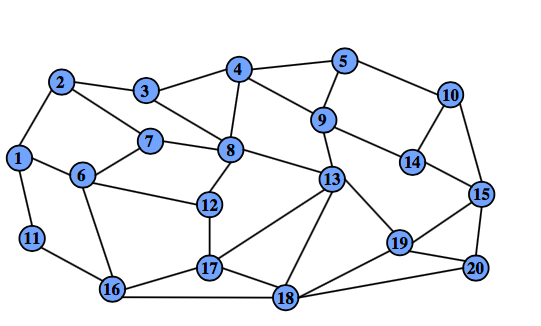
\includegraphics[scale=0.5]{images/routes.png}
\caption{Estructura de una red de emergencia}
\end{figure}
	
    A partir de la observación de desastres como huracanes e inundaciones Se afirma que la velocidad de viaje en cada arco de la red decrece con el impacto del desastre \cite{tufekci1995integrated}. La disminución de la velocidad de viaje es dependiente de la posición del arco, el tipo de desastre y otros.  Sin pérdida de generalidad, la función de velocidad puede representarse como:
\begin{equation}
	  s_{ij}(t) = s_{ij}^0 \cdot \alpha_{ij} \cdot e^{-\beta_{ij} \cdot t}
\end{equation}
donde \(\alpha_{ij}\) y \(\beta_{ij}\) son los parámetros decrecientes que determinan la disminución de la velocidad del viaje \(s_{ij}(t)\), \(\alpha_{ij}\) y \(\beta_{ij}\) pueden ser estimados de acuerdo a factores como la distancia desde arco $(v_i,v_j)$ al centro del desastre, la vulnerabilidad del arco, el tipo de desastre, entre otros.
	\item Sea \(t_{ij}\) el tiempo necesario para viajar a través del arco $(v_i,v_j)$, se calcula como $t_{ij}=t_j-t_i$.
	\item Sea $x_{ij}$ es variable de decisión del modelo $x_{ij} = 1 $ cuando el arco $(v_i,v_j)$ es incluido en el camino y $x_{ij} = 0 $ cuando el arco $(v_i,v_j)$ no es incluido en el camino.
	\item P denota el camino realizado, o sea la secuencia de nodos en la redes que se elige. Sea $p_k$ el número de la secuencia del nodo $v_{p_k}$	en la red, entonces P puede ser presentado como $(v_{p_1},v_{p_2},\cdots,v_{p_k},\cdots,v_{p_K})$ donde $1\leq p_k \leq n$ y k es la secuencia del nodo   $v_{p_k}$ en el camino P.  P debe iniciar en el nodo inicial $p_1=1$ y $p_K=n$. Y no deben existir ciclos.
	\item Sea $ET(P,v_{p_k})$ el tiempo de viaje desde $v_{p_1}$ que termina en $v_{p_k}$ a lo largo de $(v_{p_1},v_{p_2},\cdots,v_{p_k})$ donde $1\leq p_k \leq n$. A partir de esto se determina que:
	\begin{equation}
		ET(P,v_{p_k})= \sum_{m=1}^{k-1} t_{p_mp_{m+1}} = (t_{p_2} - t_{p_1}) +(t_{p_3} - t_{p_2}) + \cdots + (t_{p_k} - t_{p_{k-1}}) = t_{p_k}
	\end{equation}
	

\end{itemize}
 A partir de lo anterior podemos calcular el tiempo de un camino, dado que:
\begin{equation}\label{borde}
	  t_{p_1} = t_1 = 0
\end{equation} 
 
\begin{equation}\label{int}
\int_{t_{p_{k-1}}}^{t_{p_k}} s_{p_{k-1}p_k}(t)dt = l_{p_{k-1}p_k} \text{  \(2 \leq k \leq  K\)}
 \end{equation}
 
En la ecuación \eqref{int} conocemos el límite inferior de la integral, el integrando $ s_{p_{k-1}p_k}$ y el resultado de $ l_{p_{k-1}p_k} $, por lo tanto, se puede obtener el límite superior $t_{p_k}$.
Por recursividad se puede obtener los valores de $t_{p_k}$ para los nodos $v_{p_k}$ con  $1\leq p_k \leq n$.

\subsection{Modelo matemático}
%Uno o m\'as modelos matem\'aticos para el problema, idealmente indicando elp espacio de b\'usqueda para cada uno.
A continuación se resume la notación utilizada para modelar el problema \textit{route selection for emergency logistics management}
\subsubsection{Notación}
\begin{itemize}
	\item $i$  indice para los nodos en la red
	\item $v_i$ nodo $i$ de la red
 	\item $(i,j)$ arco desde i a j
	\item $x_{ij}$ variable de decisión del modelo, $x_{ij} = 1 $ cuando el arco de los nodos $(v_i,v_j)$ es incluido en el camino, en caso contrario $x_{ij} = 0$
	\item $l_{ij}$ largo del arco desde i a j
	\item $s^{o}_{ij}$  velocidad entre los arcos $(v_i, v_j)$ en condiciones normales
	\item $s_{ij}(t)$ velocidad entre los arcos $(v_i, v_j)$ en el tiempo $t$
	\item $\alpha_{ij}$ parámetro decreciente para manipular la velocidad           
	\item $\beta_{ij}$ parámetro decreciente para manipular la velocidad             
	\item $t_{ij}$ tiempo necesario para viajar entre i y j                      
\end{itemize}

Considerando lo descrito por \cite{southworth1991regional,cova2003network} se diseñan dos modelos con distintos objetivos: el primero busca la minimización del tiempo y el segundo busca múltiples objetivos: la minimización del tiempo y de la cantidad de nodos en la ruta.
\subsubsection{Minimización del tiempo:} 

La formulación del \textit{route selection for emergency logistics management} se describe de la siguiente manera:

El objetivo del modelo es minimizar el tiempo empleado en el camino. Las ecuaciones \eqref{7}, \eqref{8} y \eqref{9} son parte de la fórmula de recursión del tiempo total para el camino. En la ecuación \eqref{speed} la función decreciente de la velocidad de viaje en el arco $(v_i,v_j)$. La restricción \eqref{full} asegura un camino factible desde $v_1$ hasta $v_n$ y la restricción \eqref{circles} asegura que no existan ciclos.

\begin{equation}
	 \text{mín} \sum_{i=1}^{n}\sum_{j=1}^{n} t_{ij} \cdot x_{ij}
\end{equation}

\begin{equation}\label{7}
  \int_{t_i}^{t_j} s_{ij}(t)dt = l_{ij}
\end{equation}
\begin{equation}\label{8}
  t_{ij} = t_j - t_i
\end{equation}
\begin{equation}\label{9}
t_1 =0
\end{equation}
\begin{equation}\label{speed}
  s_{ij}(t) = s_{ij}^0 \cdot \alpha_{ij} \cdot e^{-\beta_{ij}\cdot t}
\end{equation}

\begin{equation}\label{full}
	\sum_{\substack{j=1\\
                  j \neq i}}^n x_{ij} - \sum_{\substack{j=1\\
                  j \neq i}}^{n} x_{ji} = \begin{cases}
1 & i=1\\
-1 & i=n \\
0 & eoc
\end{cases}
\end{equation}



\begin{equation}\label{circles}
	\sum_{\substack{j=1\\
                  j \neq i}}^n x_{ij} = \begin{cases}
\leq 1 & i\neq n\\
=0 & i=n 
\end{cases}
\end{equation}

\begin{equation}
	x_{ij} = 0,1;i=1,2,\cdots,n;j=1,2,\cdots,n
\end{equation}

%\subsubsection{Multi-objetivo para \textit{route selection for emergency logistics management} }
%
%\cite{southworth1991regional,cova2003network} han mostrado que la mayor congestión sucede en las intersecciones de dos arcos en una red de emergencia, cuando se viaja en un camino con menor número de arcos es más fácil y rápido seguir el camino. La complejidad del camino puede obtenerse por el número de arcos incluídos en un camino. 
%
%
%\begin{equation}\label{f_1}
%	 \text{mín}  f_1 = \sum_{i=1}^{n}\sum_{j=1}^{n} t_{ij}x_{ij}
%\end{equation}
%
%
%\begin{equation}\label{f_2}
%	 \text{mín}  f_2 = \sum_{i=1}^{n}\sum_{j=1}^{n} x_{ij}
%\end{equation}
%
%Las restricciones se heredan del modelo anterior.
\section{Estado del Arte}

%Lo m\'as importante que se ha hecho hasta ahora con relaci\'on al problema. Deber\'ia responder preguntas como las siguientes:
%?`cuando surge?, ?`qu\'e m\'etodos se han usado para resolverlo?, ?`cuales son los mejores algoritmos que se han creado hasta
%la fecha?, ?`qu\'e representaciones han tenido los mejores resultados?, ?`cu\'al es la tendencia actual?, tipos de movimientos,
%heur\'isticas, m\'etodos completos, tendencias, etc... Puede incluir gr\'aficos comparativos, o explicativos.\\

\textit{Route selection for emergency logistics management} es uno de los problemas fundamentales de logística. En los recientes años, los frecuentes desastres naturales ha incentivado la investigación en el área. El primer trabajo sobre enrutamiento de vehículos fue propuesto por \cite{dantzig1959truck} donde se optimiza el reparto de combustible usando camiones que distribuyen desde una terminal hasta múltiples estaciones de servicios. En \cite{ozdamar2004emergency} se propone un modelo para el diseño de rutas en caso emergencias, el objetivo es minimizar la demanda insatisfecha en la ruta planeada. El plan logístico de emergencia incluye los puntos óptimos donde recoger y entregar los materiales en las rutas, estas rutas son regeneradas mientras nuevos materiales y modos de transportes se vuelven disponibles, pero este trabajo no considera que el tiempo de viaje puede variar según el efecto de la catástrofe sobre los caminos.
Según \cite{farahmand1997application,tufekci1995integrated} es importante considerar el efecto de la catástrofe sobre los caminos dado que las condiciones de viaje entre los nodos pueden verse fuertemente afectadas por la extensión del desastre, especialmente en desastres como huracanes e inundaciones que se extienden en tiempo y espacio.
%detalles feronoma, conocimiento heuristico, calidad => tiempo
Otros trabajos como \cite{Yuan20091081} construyeron un modelo para expresar el efecto de la extensión de un desastre en los caminos, el efecto es representado con la variación de la velocidad de viaje. Para la resolución de este problema se utilizan dos técnicas: la primera basada en el algoritmo de Dijkstra, donde la idea es encontrar el camino más corto paso a paso y la técnica es un algoritmo basado en \textit{Ant system}, el conocimiento heuristico para el movimiento es la función de velocidad $s_{ij}(t) = s_{ij}^0 \cdot \alpha_{ij} \cdot e^{-\beta_{ij}\cdot t}$ si que un camino posible entre el nodo $i$ y $j$.

sin mostrar valores de los parámetros. Los resultados experimentales fueron realizados con 20 nodos evaluando las dos técnicas: Dijkstra y ACO, donde ACO obtuvo mejores resultados en comparación con Dijkstra. Además ACO obtuvo rutas con menor tiempo de viaje de la instancia sin especificar el tiempo de ejecución. Las instancias utilizada por Dijkstra y ACO son las mismas.\\
En \cite{zhang2013route} se propone un algoritmo inspirado en la biología observando y modelando el comportamiento de las ameboides para calcular las rutas de emergencia donde la velocidad de los arcos es variable. Los experimentos fueron realizados con 20 nodos donde se obtuvieron las mejores soluciones respecto a tiempo de las instancias sin especifica el tiempo de ejecución.\\
Por otra parte, investigaciones relacionadas \cite{southworth1991regional,cova2003network} han mostrado que las mayores congestiones de un desastre son producidas en las intersecciones de dos arcos en una ruta de emergencia, produciendo un nuevo problema \textit{Lane-based routing} donde la estrategia busca eliminar los cruces en las intersecciones. 
Además, en \cite{xie2011lane} se propone un método para resolver una evacuación considerando el cruce de intersecciones (\textit{lane-based}), la técnica utilizada es tabú search y relajación lagrangiana, a diferencia de \textit{route selection for emergency logistics management} modela el número de vías en un camino (camino con varias vías), capacidad de flujo del camina y demanda del nodo, siendo un problema mayor complejidad. El algoritmo es aplicado en un red de 100 nodos modelando la evacuación Monticello, Minnesota. El algoritmo converge entre las 350 y 450 iteraciones.
En \cite{stepanov2009multi} se propone un modelo de programación entera para determinar la ruta óptima en caso de evacuación modelando la capacidad de los refugios donde las personas serán evacuadas, además modela la posibilidad de bloqueo por congestión. El algoritmo es evaluado en una instancia con tres áreas a evacuar, la red se encuentra compuesta de 31 nodos.
En \cite{tan2011if} entrega rutas de evacuación incluyendo planes para la distribución de vehículos considerando: las capacidades, emisiones de gases, costos económicos, entre otros. Estos son trabajados por un modelo difuso de evaluación basado en parámetros. Las simulaciones son realizadas con 8 nodos. Dada la incertidumbre y complejidad del ambiente en la emergencia, estos modelos tienen serias limitaciones en manejar el proceso de evaluación basado en los comportamientos individuales \cite{liu2016evacuation}.\\

En \cite{rahman2007feasible} describe una emergencia considerando múltiples aspectos: minimizar el camino de salida en un edificio con múltiples salidas y niveles, utiliza \textit{Ant Colony System} modificado para encontrar una ruta factible para resolver el problema. Define distintos tipos de agentes según el sector: agente señal de salida, agente de pasillo, agente de escaleras y agente habitante. La evaluación es realizada en uno edificio de la Universidad Tecnológica de Petronas en Malaysia, el edificio tiene cuatro pisos, cada piso con cuatro bloques de piezas y cada bloque tiene doce piezas. La función a minimizar en el tiempo de evacuación $T_{clear}$ y el número de ocupantes seguros. El autor realiza una comparación con el software IntelSign y el algoritmo propuesto. Finalmente el algoritmo obtiene mejores resultados que IntelSign respecto al tiempo de evacuación total.
En \cite{zong2010multi} se presenta un algoritmo \textit{ant colony system} multi-objetivo para resolver problemas de evacuaciones de automóviles y peatones  considerando los aspectos como congestión, número de automóviles y peatones. El autor considera dos objetivos: minimizar el tiempo total de la evacuación y minimizar el número de arcos en camino total. Los experimentos son realizados con una simulación del estadio \textit{Wuhan Sports Center} representada por 157 nodos dentro del estadio, 319 caminos fuera del estadio y 8 zonas de seguridad. Las parámetros utilizados son: $\alpha=2$, $\beta=3$, $\rho=0.7$, $w=1$, $k=0.5$
Como continuación al trabajo anterior en \cite{zong2010multiflow} se utiliza modelo \textit{multi-ant colony system} para considerar la evacuación de automóviles y peatones. En este caso, \textit{Multi-ant colony system} \cite{gambardella1999macs}utilizada dos tipos de hormigas, una colonia encargada en la evacuación de peatones y otra colonia para la evacuación de vehículos, ambas colonias pueden comunicarse utilizando las feromonas. Los experimentos son realizados en las mismas condiciones y mismos parámetros, finalmente el autor concluye que el algoritmo MACS puede obtener mejores soluciones en comparación a ACS.
En \cite{forcael2014ant} se desarrolla un ACO para optimizar evacuaciones de personas en caso de tsunami considerando la seguridad, la calidad y la pendiente de los caminos. La simulación se realiza en la ciudad de Penco Chile que se representa con 67 nodos y dos zonas de seguridad. El autor hace un análisis para una simulación especifica (desde nodo 16 hacia la zona de seguridad 2), mostrando que el algoritmo alcanza su mejor valor a las 50 iteraciones y se mantiene estable después de 300 iteraciones utilizando 100 hormigas. Luego, realiza una simulación con personas reales para validar el modelo, agrupa dos grupos de personas de un total de 34 adultos jóvenes: el primer grupo posicionado de manera aleatoria sin ninguna información sobre rutas de escape y el segundo grupo posicionado de manera aleatoria con información de las rutas construídas por el algoritmo. El autor concluye que los tiempos del modelo y la realidad no presentan diferencias significativas y por lo tanto el modelo utilizado permite modelar efectivamente una evacuación en caso de tsunami. Realizando una comparación de tiempos entre los grupos existen diferencias a favor del modelo, presentando hasta 7 minutos menos de tiempo necesario para la evacuación. \\
En \cite{ohta2016improved} se propone un algoritmo \textit{Max-Min Ant System}, que utiliza una nueva feromona llamada desodorante que elimina la feromona común de ACO cuando un camino peligroso ha sido encontrado, el objetivo de esta nueva  feromona es poder entregar un mayor nivel de seguridad. La evaluación se realiza con un mapa de distrito de Shinjuku en Tokyo representada una matriz de 200x200, donde cada celda se categoriza como: Camino, área segura, área peligrosa y área no utilizable (murallas, edificios, etc). El área peligrosa aumenta de acuerdo al porcentaje de personas evaluadas en el lugar. La evaluación se realiza con 500 iteraciones sin información de parámetros, finalmente el autor realiza una comparación con \textit{Ant system} y concluye que el algoritmo propuesto permite evitar a nuevas zonas inseguras.
En \cite{liu2016evacuation} se propone la utilización de \textit{quantum ant colony algorithm (QACA)} utilizando conceptos y reglas de computación cuántica y ACO. El autor modela la evacuación desde una zona de peligro hacia una zona segura, cada zona presenta un número determinado de nodos y cada nodo tiene una capacidad máxima. El autor busca minimizar el tiempo de la evacuación y la densidad de personas en los nodos de la zona de seguridad. La evacuación se realiza en una red ficticia con 50 nodos donde se compara los resultados con una técnica ACO, el autor concluye que los resultados obtenido por el algoritmo propuesto utilizando QACA presentan mejores soluciones considerando el tiempo total de la evacuación en comparación a ACO.\\
%En \cite{fang2011hierarchical} se propone la utilización de \textit{} Los experimentos son realizados con una simulación del estadio \textit{Wuhan Sports Center} que se representa 157 nodos dentro del estadio, 319 caminos fuera del estadio y 8 zonas de seguridad.
%evolutivo
%En \cite{saadatseresht2009evacuation} se utiliza un algoritmo evolutivo multi-objetivo y sistemas de información geográfica para realizar una estrategia de evacuación. En el modelo se busca maximizar la capacidad de las áreas seguras y minimizar la distancia a ellos utilizando el algoritmo \texttt{NSGA-II} \cite{deb2002fast}. \\
En \cite{izquierdo2009forecasting,zheng2012modeling} se propone el uso de\textit{particle swarm optimization (PSO)} para la evacuación de peatones en áreas con alto trafico, el uso de PSO busca poder utilizar la inteligencia individual y colectiva de los agentes.
En \cite{zong2014conflict} se presenta un modelo \textit{discrete particle swarm optimization (DPSO)} para la evacuación de peatones y vehículos en caso de emergencia realizando un modelado y simulación de los movimientos de evacuación e interacción entre peatones y vehículos.  Los experimentos son realizados utilizando el estadio \textit{Wuhan Sports Center} que se representa con 157 nodos dentro del estadio, 319 caminos fuera del estadio y 8 zonas de seguridad. En la emergencia se realiza una evacuación de 10.000 peatones y 1.000 vehículos y se compra con ACO y MACO propuesto en \cite{zong2010multi,zong2010multiflow} utilizando los siguientes parámetros para ellos $\alpha=2$, $\beta=3$, $\rho=0.7$, $Q=100$, $k=1$ y el coeficiente de comunicación $\lambda=0.5$ para MACO. Los resultados muestran 	que los tiempos para los algoritmos PSO son mejores y el autor concluye que es debido a los mecanismos de aprendizaje de PSO. Por otro lado, el autor concluye que MACO presenta mejores resultados que ACO.
%explicar maco

\section{Descripción propuesta}
\subsection{Representación}
Notación:
\begin{itemize}
	\item $i$ indice para los nodos en la red
	\item $v_i$ nodo $i$ de la red
 	\item $(i,j)$ arco desde i a j
	\item $x_{ij}$ variable de decisión del modelo, $x_{ij} = 1 $ cuando el arco de los nodos $(v_i,v_j)$ es incluido en el camino, en caso contrario $x_{ij} = 0$
	\item $l_{ij}$ largo del arco desde i a j
	\item $s^{o}_{ij}$  velocidad entre los arcos $(v_i, v_j)$ en condiciones normales
	\item $s_{ij}(t)$ velocidad entre los arcos $(v_i, v_j)$ en el tiempo $t$
	\item $\alpha_{ij}$ parámetro decreciente para manipular la velocidad           
	\item $\beta_{ij}$ parámetro decreciente para manipular la velocidad             
	\item $t_{ij}$ tiempo necesario para viajar entre i y j                      
\end{itemize}

La formulación del \textit{route selection for emergency logistics management} se describe de la siguiente manera:

El objetivo del modelo es minimizar el tiempo empleado en el camino. Las ecuaciones \eqref{7}, \eqref{8} y \eqref{9} son parte de la fórmula de recursión del tiempo total para el camino. En la ecuación \eqref{speed} la función decreciente de la velocidad de viaje en el arco $(v_i,v_j)$. La restricción \eqref{full} asegura un camino factible desde $v_1$ hasta $v_n$,la restricción \eqref{circles} asegura que no existan ciclos y \eqref{full} muestra los dominios de las variables.

\begin{equation}
	 \text{mín} \sum_{i=1}^{n}\sum_{j=1}^{n} t_{ij} \cdot x_{ij}
\end{equation}

\begin{equation}\label{7}
  \int_{t_i}^{t_j} s_{ij}(t)dt = l_{ij}
\end{equation}
\begin{equation}\label{8}
  t_{ij} = t_j - t_i
\end{equation}
\begin{equation}\label{9}
t_1 =0
\end{equation}
\begin{equation}\label{speed}
  s_{ij}(t) = s_{ij}^0 \cdot \alpha_{ij} \cdot e^{-\beta_{ij}\cdot t}
\end{equation}

\begin{equation}\label{full}
	\sum_{\substack{j=1\\
                  j \neq i}}^n x_{ij} - \sum_{\substack{j=1\\
                  j \neq i}}^{n} x_{ji} = \begin{cases}
1 & i=1\\
-1 & i=n \\
0 & eoc
\end{cases}
\end{equation}



\begin{equation}\label{circles}
	\sum_{\substack{j=1\\
                  j \neq i}}^n x_{ij} = \begin{cases}
\leq 1 & i\neq n\\
=0 & i=n 
\end{cases}
\end{equation}

\begin{equation}
	x_{ij} = 0,1;i=1,2,\cdots,n;j=1,2,\cdots,n
\end{equation}
\subsection{Operadores/Movimientos}
La decisión para la selección del siguiente nodo se realiza en base al movimiento  definido por:
\begin{equation}
j = \begin{cases} arg max_{u \in S_{k}(i)} \{ [\tau(i,u)]^\alpha [\eta(i,u)]^\beta\} &\mbox{if } q \leq q_0 \\ 
J & otherwise \end{cases} 
\end{equation}

Donde $J \in J_i^k$ se elige según la probabilidad:

	\begin{equation}
		P_{ij}^k(t) = \frac{[\tau_{ij}(t)]^{\alpha_a}[\eta_{ij}]^{\beta_a}}{\sum_{h \in J_i^k } [\tau_{ij}(t)]^{\alpha_a}[\eta_{ij}]^{\beta_a}}
	\end{equation}
	
Para la sección de siguiente nodo se considera la heurística del tiempo expresada por $\eta = \frac{1}{tiempo\_tour}$.
En caso que el nodo sea un nodo seguro se selecciona el nodo y se finaliza la construcción del camino.
%todo: descripcion de cada proceso
\subsection{Descripción de cada proceso}
\subsection{Pseudocódigo general}
En general, el algoritmo implementado está basado en el algoritmo Ant Colony System \cite{dorigo1997ant}. En \ref{alg} se muestra un pseudocógido del algoritmo \\
\begin{algorithm}[]
\label{alg}

 \KwData{Algoritmo propuesto}
 inicializar\;
 \For{cada arco (i,j)}{
 	$\tau_{ij}(0) = \tau_{0}$
 }
 \For{k=1 hasta n}{
 	Ubique la hormiga $k$ en el primer nodo
 }
 Sea $T+$ el tour más corto encontrado desde el inicio\;
 \For{t=1 hasta el número de iteraciones}{
 \For{k=1 hasta m}{
 \While{no se complete el tour}{
  \eIf{si existe un nodo j $\in$ cl }{
   Elegir un nodo $j$, $j \in j_{i}^{k}$ entre $cl$ nodos de la lista\;
\begin{equation*}
j = \begin{cases} arg max_{u \in J_{i}^{k}} \{ [\tau_{iu}(t))]^\alpha [\eta_{iu}]^\beta\} &\mbox{if } q \leq q_0 \\ 
J & otherwise \end{cases}
\end{equation*}
	Donde $J \in J_i^k$ se elige según la probabilidad\;
	\begin{equation}
		P_{ij}^k(t) = \frac{[\tau_{ij}(t)]^{\alpha}[\eta_{ij}]^{\beta}}{\sum_{h \in J_i^k } [\tau_{ih}(t)]^{\alpha}[\eta_{ih}]^{\beta}}
	\end{equation}
Y donde $i$ es el nodo actual.
%else
   }
   {
   elegir el nodo $j \in J_{i}^{k}$ más cercana.
  }
 Luego se actualiza la feromona\;
\begin{equation}
	t_{ij}(t) = (1-\rho)t_{ij}(t) + \rho \tau_0
\end{equation}
 }
 %while tour
 Calcular el tiempo $T_k$ del tour de la hormiga $k$
 }
 Salvar la mejor solución $T^{+}$ encontrada hasta el momento
 %for hormigas
 
 \For{cada arco (i,j) $\in T^{+}$ }{
\begin{equation}
	t_{ij}(t) = (1-\rho)t_{ij}(t) + \rho \Delta \tau_{ij}(t)	
\end{equation}
	donde $\tau_{ij}(t) = \frac{1}{T^{+}}$
 }
 }
 %for iteraciones
 \caption{Algoritmo ACS.}
\end{algorithm}
\subsection{Listado de parámetros del algoritmo}

A continuación se presenta los parámetros utilizados por el algoritmo.
\begin{itemize}
\item Número de iteraciones: $loops=2000$
\item Tamaño de la lista candidata $cl=15$
\item Número de hormigas $M=[6,88]$
\item Parámetro ACS $\alpha_{ant}=[1.29, 4.23]$
\item Parámetro ACS $\beta_{ant}=[2.5,9.83]$
\item Selección $q_0=[0.08,0.94]$
\item Evaporación $\rho=[0.11,0.97]$
\item Feromona inicial $\tau_{0}=0.1$
\end{itemize}



\subsection{Instancias de pruebas}



En el  \cite{Yuan20091081} se presenta un red de 20 nodos divididos en 3 áreas que se muestra en la figura \ref{area3}. En cada área los parámetros son generados de forma aleatoria, los cuales se observan en el cuadro \ref{table:intervalo}. Para el desastre 0 es una situación sin ningún desastre y el desastre 4 es situación más compleja. Para las instancias propuesta por \cite{Yuan20091081} se considera que el nodo 20 es un nodo seguro.

\begin{figure}[H]
\centering
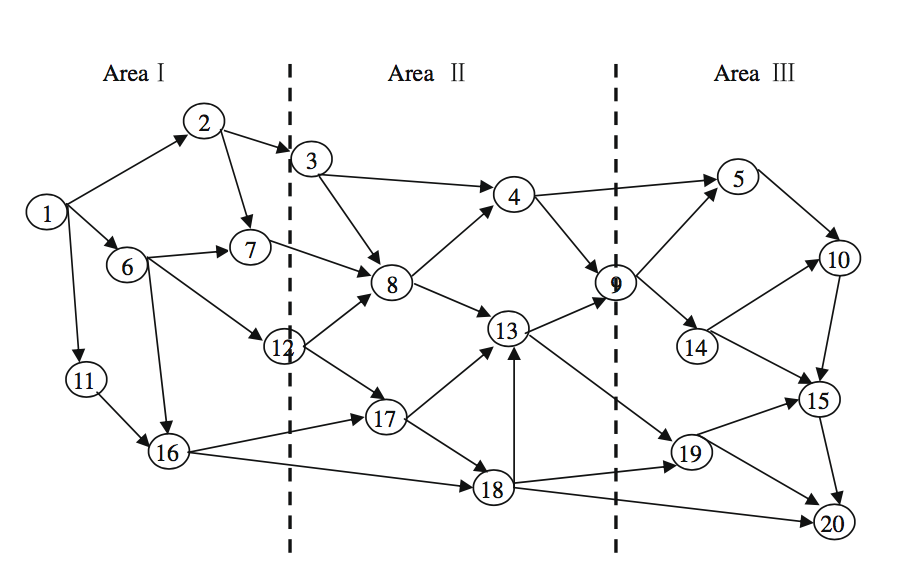
\includegraphics[scale=0.5]{images/areas.jpg}
\caption{División de una red de emergencia}\label{area3}

\end{figure}

En los cuadros \ref{grade1}, \ref{grade2}, \ref{grade3} y \ref{grade4} se muestran los valores correspondientes al nodo $i$ y nodo $j$. $l_{i,j}$ $s_{i,j}^0$, $\alpha_{ij}$ y $\beta_{ij}$ según los distintos grados de desastre.



\begin{table}[H]
\centering
\begin{tabular}{|l|l|l|l|}
\hline
Tipo & Área I & Área II & Área III \\ \hline
Desastre 0 & $\alpha=1$,$\beta=0$ & $\alpha=1$,$\beta=0$ & $\alpha=1$,$\beta=0$ \\ \hline
Desastre 1 & $\alpha \in (0.9,1.0)$ $\beta \in (0.00,0.05)$ & $\alpha=1$,$\beta=0$ & $\alpha=1$,$\beta=0$ \\ \hline
Desastre 2 & $\alpha \in (0.8,0.9)$ $\beta \in (0.05,0.10)$ & $\alpha \in (0.9,1.0)$ $\beta \in (0.00,0.05)$ & $\alpha=1$,$\beta=0$ \\ \hline
Desastre 3 & $\alpha \in (0.7,0.8)$ $\beta \in (0.10,0.15)$ & $\alpha \in (0.8,0.9)$ $\beta \in (0.05,0.10)$ & $\alpha \in (0.9,1.0)$ $\beta \in (0.00,0.05)$ \\ \hline
Desastre 4 & $\alpha \in (0.6,0.7)$ $\beta \in (0.15,0.20)$ & $\alpha \in (0.7,0.8)$ $\beta \in (0.10,0.15)$ & $\alpha \in (0.8,0.9)$ $\beta \in (0.05,0.10)$ \\ \hline
\end{tabular}
\caption{Intervalos de los parametros por área}\label{table:intervalo}
\end{table}




\begin{table}[H]
\centering
\begin{tabular}{|l|l|l|l|l|l|}
\hline
inicio & fin & $l_{i,j}$ & $s_{i,j}^0$ & $\alpha_{i,j}$ & $\beta_{i,j}$ \\ \hline
1 & 2 & 50 & 100 & 0.9222 & 0.0381 \\ \hline
1 & 6 & 30 & 60 & 0.9193 & 0.0143 \\ \hline
1 & 11 & 70 & 110 & 0.9022 & 0.0499 \\ \hline
2 & 3 & 30 & 60 & 0.9904 & 0.0277 \\ \hline
2 & 7 & 40 & 70 & 0.9857 & 0.0305 \\ \hline
6 & 7 & 30 & 65 & 0.9577 & 0.0123 \\ \hline
6 & 12 & 60 & 105 & 0.906 & 0.0399 \\ \hline
6 & 16 & 100 & 115 & 0.9049 & 0.0353 \\ \hline
7 & 8 & 40 & 90 & 0.9153 & 0.0436 \\ \hline
11 & 16 & 30 & 70 & 0.9967 & 0.0089 \\ \hline
16 & 17 & 80 & 115 & 0.964 & 0.0491 \\ \hline
16 & 18 & 110 & 120 & 0.9294 & 0.0327 \\ \hline
3 & 4 & 80 & 100 & 1 & 0 \\ \hline
3 & 8 & 60 & 95 & 1 & 0 \\ \hline
4 & 5 & 110 & 120 & 1 & 0 \\ \hline
4 & 9 & 40 & 75 & 1 & 0 \\ \hline
5 & 10 & 60 & 110 & 1 & 0 \\ \hline
8 & 4 & 40 & 85 & 1 & 0 \\ \hline
8 & 13 & 30 & 75 & 1 & 0 \\ \hline
9 & 5 & 70 & 110 & 1 & 0 \\ \hline
9 & 14 & 40 & 90 & 1 & 0 \\ \hline
10 & 15 & 50 & 105 & 1 & 0 \\ \hline
12 & 8 & 30 & 65 & 1 & 0 \\ \hline
12 & 17 & 40 & 100 & 1 & 0 \\ \hline
13 & 9 & 30 & 80 & 1 & 0 \\ \hline
13 & 19 & 110 & 120 & 1 & 0 \\ \hline
14 & 10 & 80 & 115 & 1 & 0 \\ \hline
14 & 15 & 60 & 105 & 1 & 0 \\ \hline
15 & 20 & 30 & 90 & 1 & 0 \\ \hline
17 & 13 & 40 & 80 & 1 & 0 \\ \hline
17 & 18 & 40 & 75 & 1 & 0 \\ \hline
18 & 13 & 60 & 115 & 1 & 0 \\ \hline
18 & 19 & 70 & 110 & 1 & 0 \\ \hline
18 & 20 & 120 & 120 & 1 & 0 \\ \hline
19 & 15 & 40 & 75 & 1 & 0 \\ \hline
19 & 20 & 70 & 105 & 1 & 0 \\ \hline

\end{tabular}
\caption{Parámetros para un desastre grado 1}
\label{grade1}
\end{table}


\begin{table}[H]
\centering
\begin{tabular}{|l|l|l|l|l|l|}
\hline
inicio & fin & $l_{i,j}$ & $s_{i,j}^0$ & $\alpha_{i,j}$ & $\beta_{i,j}$ \\ \hline
1 & 2 & 50 & 100 & 0.9222 & 0.0381 \\ \hline
1 & 6 & 30 & 60 & 0.9193 & 0.0143 \\ \hline
1 & 11 & 70 & 110 & 0.9022 & 0.0499 \\ \hline
2 & 3 & 30 & 60 & 0.9904 & 0.0277 \\ \hline
2 & 7 & 40 & 70 & 0.9857 & 0.0305 \\ \hline
6 & 7 & 30 & 65 & 0.9577 & 0.0123 \\ \hline
6 & 12 & 60 & 105 & 0.906 & 0.0399 \\ \hline
6 & 16 & 100 & 115 & 0.9049 & 0.0353 \\ \hline
7 & 8 & 40 & 90 & 0.9153 & 0.0436 \\ \hline
11 & 16 & 30 & 70 & 0.9967 & 0.0089 \\ \hline
16 & 17 & 80 & 115 & 0.964 & 0.0491 \\ \hline
16 & 18 & 110 & 120 & 0.9294 & 0.0327 \\ \hline
3 & 4 & 80 & 100 & 0.9153 & 0.0216 \\ \hline
3 & 8 & 60 & 95 & 0.9562 & 0.0114 \\ \hline
4 & 5 & 110 & 120 & 0.989 & 0.0281 \\ \hline
4 & 9 & 40 & 75 & 0.9984 & 0.0386 \\ \hline
8 & 4 & 40 & 85 & 0.9746 & 0.0376 \\ \hline
8 & 13 & 30 & 75 & 0.9999 & 0.0222 \\ \hline
12 & 8 & 30 & 65 & 0.9345 & 0.0044 \\ \hline
12 & 17 & 40 & 100 & 0.9846 & 0.0228 \\ \hline
13 & 9 & 30 & 80 & 0.9094 & 0.0264 \\ \hline
13 & 19 & 110 & 120 & 0.9326 & 0.0151 \\ \hline
17 & 13 & 40 & 80 & 0.9077 & 0.035 \\ \hline
17 & 18 & 40 & 75 & 0.947 & 0.0344 \\ \hline
18 & 13 & 60 & 115 & 0.9669 & 0.0202 \\ \hline
18 & 19 & 70 & 110 & 0.953 & 0.0059 \\ \hline
18 & 20 & 120 & 120 & 0.9278 & 0.0021 \\ \hline
5 & 10 & 60 & 110 & 1 & 0 \\ \hline
9 & 5 & 70 & 110 & 1 & 0 \\ \hline
9 & 14 & 40 & 90 & 1 & 0 \\ \hline
10 & 15 & 50 & 105 & 1 & 0 \\ \hline
14 & 10 & 80 & 115 & 1 & 0 \\ \hline
14 & 15 & 60 & 105 & 1 & 0 \\ \hline
15 & 20 & 30 & 90 & 1 & 0 \\ \hline
19 & 15 & 40 & 75 & 1 & 0 \\ \hline
19 & 20 & 70 & 105 & 1 & 0 \\ \hline
\end{tabular}
\caption{Parámetros para un desastre grado 2}
\label{grade2}
\end{table}

\begin{table}[H]
\centering
\begin{tabular}{|l|l|l|l|l|l|}
\hline
inicio & fin & $l_{i,j}$ & $s_{i,j}^0$ & $\alpha_{i,j}$ & $\beta_{i,j}$ \\ \hline
1 & 2 & 50 & 100 & 0.7544 & 0.1026 \\ \hline
1 & 6 & 30 & 60 & 0.7666 & 0.1394 \\ \hline
1 & 11 & 70 & 110 & 0.7561 & 0.1276 \\ \hline
2 & 3 & 30 & 60 & 0.7071 & 0.1089 \\ \hline
2 & 7 & 40 & 70 & 0.7527 & 0.1277 \\ \hline
6 & 7 & 30 & 65 & 0.7001 & 0.1062 \\ \hline
6 & 12 & 60 & 105 & 0.7145 & 0.1209 \\ \hline
6 & 16 & 100 & 115 & 0.7234 & 0.1361 \\ \hline
7 & 8 & 40 & 90 & 0.7242 & 0.108 \\ \hline
11 & 16 & 30 & 70 & 0.7378 & 0.1281 \\ \hline
16 & 17 & 80 & 115 & 0.7048 & 0.1197 \\ \hline
16 & 18 & 110 & 120 & 0.7639 & 0.1365 \\ \hline
3 & 4 & 80 & 100 & 0.8912 & 0.0844 \\ \hline
3 & 8 & 60 & 95 & 0.8242 & 0.0571 \\ \hline
4 & 5 & 110 & 120 & 0.8773 & 0.0552 \\ \hline
4 & 9 & 40 & 75 & 0.8678 & 0.099 \\ \hline
8 & 4 & 40 & 85 & 0.8801 & 0.067 \\ \hline
8 & 13 & 30 & 75 & 0.8425 & 0.0987 \\ \hline
12 & 8 & 30 & 65 & 0.8383 & 0.0543 \\ \hline
12 & 17 & 40 & 100 & 0.8785 & 0.0786 \\ \hline
13 & 9 & 30 & 80 & 0.8551 & 0.0707 \\ \hline
13 & 19 & 110 & 120 & 0.873 & 0.057 \\ \hline
17 & 13 & 40 & 80 & 0.8191 & 0.0778 \\ \hline
17 & 18 & 40 & 75 & 0.8555 & 0.0781 \\ \hline
18 & 13 & 60 & 115 & 0.8965 & 0.0653 \\ \hline
18 & 19 & 70 & 110 & 0.8967 & 0.0694 \\ \hline
18 & 20 & 120 & 120 & 0.8551 & 0.0948 \\ \hline
5 & 10 & 60 & 110 & 0.9476 & 0.0343 \\ \hline
9 & 5 & 70 & 110 & 0.9806 & 0.0484 \\ \hline
9 & 14 & 40 & 90 & 0.9984 & 0.0219 \\ \hline
10 & 15 & 50 & 105 & 0.9937 & 0.0091 \\ \hline
14 & 10 & 80 & 115 & 0.9334 & 0.0486 \\ \hline
14 & 15 & 60 & 105 & 0.9966 & 0.022 \\ \hline
15 & 20 & 30 & 90 & 0.9517 & 0.0363 \\ \hline
19 & 15 & 40 & 75 & 0.9547 & 0.0265 \\ \hline
19 & 20 & 70 & 105 & 0.9849 & 0.029 \\ \hline
\end{tabular}
\caption{Parámetros para un desastre grado 3}\label{grade3}
\end{table}


\begin{table}[H]
\centering
\begin{tabular}{|l|l|l|l|l|l|}
\hline
inicio & fin & $l_{i,j}$ & $s_{i,j}^0$ & $\alpha_{i,j}$ & $\beta_{i,j}$ \\ \hline
1 & 2 & 50 & 100 & 0.6396 & 0.1783 \\ \hline
1 & 6 & 30 & 60 & 0.6815 & 0.1934 \\ \hline
1 & 11 & 70 & 110 & 0.6204 & 0.1647 \\ \hline
2 & 3 & 30 & 60 & 0.6244 & 0.1698 \\ \hline
2 & 7 & 40 & 70 & 0.658 & 0.1674 \\ \hline
6 & 7 & 30 & 65 & 0.6481 & 0.1515 \\ \hline
6 & 12 & 60 & 105 & 0.6717 & 0.1957 \\ \hline
6 & 16 & 100 & 115 & 0.6706 & 0.1672 \\ \hline
7 & 8 & 40 & 90 & 0.6619 & 0.1864 \\ \hline
11 & 16 & 30 & 70 & 0.6821 & 0.1645 \\ \hline
16 & 17 & 80 & 115 & 0.6146 & 0.1858 \\ \hline
16 & 18 & 110 & 120 & 0.6625 & 0.1918 \\ \hline
3 & 4 & 80 & 100 & 0.7606 & 0.1184 \\ \hline
3 & 8 & 60 & 95 & 0.7454 & 0.1348 \\ \hline
4 & 5 & 110 & 120 & 0.7276 & 0.1178 \\ \hline
4 & 9 & 40 & 75 & 0.7686 & 0.1192 \\ \hline
8 & 4 & 40 & 85 & 0.7416 & 0.1484 \\ \hline
8 & 13 & 30 & 75 & 0.7073 & 0.132 \\ \hline
12 & 8 & 30 & 65 & 0.7911 & 0.1081 \\ \hline
12 & 17 & 40 & 100 & 0.7222 & 0.117 \\ \hline
13 & 9 & 30 & 80 & 0.7869 & 0.1274 \\ \hline
13 & 19 & 110 & 120 & 0.7775 & 0.1477 \\ \hline
17 & 13 & 40 & 80 & 0.7769 & 0.1329 \\ \hline
17 & 18 & 40 & 75 & 0.7269 & 0.1441 \\ \hline
18 & 13 & 60 & 115 & 0.711 & 0.1483 \\ \hline
18 & 19 & 70 & 110 & 0.7779 & 0.1018 \\ \hline
18 & 20 & 120 & 120 & 0.7046 & 0.127 \\ \hline
5 & 10 & 60 & 110 & 0.8334 & 0.0652 \\ \hline
9 & 5 & 70 & 110 & 0.8208 & 0.0519 \\ \hline
9 & 14 & 40 & 90 & 0.8827 & 0.0574 \\ \hline
10 & 15 & 50 & 105 & 0.8225 & 0.0678 \\ \hline
14 & 10 & 80 & 115 & 0.8736 & 0.0859 \\ \hline
14 & 15 & 60 & 105 & 0.8742 & 0.0662 \\ \hline
15 & 20 & 30 & 90 & 0.8935 & 0.0502 \\ \hline
19 & 15 & 40 & 75 & 0.8001 & 0.0811 \\ \hline
19 & 20 & 70 & 105 & 0.8535 & 0.0919 \\ \hline
\end{tabular}
\caption{Parámetros para un desastre grado 4}\label{grade4}
\end{table}


\subsection{Tablas comparativas respecto al estado del arte.}

Para comparar los resultados obtenidos por el algoritmo (Propuesto) se usarán los resultados obtenidos por  \cite{Yuan20091081} donde utiliza dos algoritmos: \textit{Best path Dijkstra} y \textit{Static shortest path}. \\

Como se muestra en los cuadros \ref{res-grade-1},\ref{res-grade-2},\ref{res-grade-3},\ref{res-grade-4} Propuesto obtiene los mejores valores posibles del problema al igual que \textit{Best path Dijkstra}. En comparación a \textit{Static shortest path}, los valores obtenidos por el algoritmo propuestos son mejores.
%todo: incluye semillas con la otra instancia
%todo: incluye convergencia
\begin{table}[H]
\centering
\begin{tabular}{|l|l|l|l|}
\hline
Algoritmo            & Camino           & Tiempo Evacuación {[}min{]} & Tiempo Ejecución {[}seg{]}\\ \hline
Best path Dijkstra   & 1 $\rightarrow$ 6$\rightarrow$12$\rightarrow$17$\rightarrow$18$\rightarrow$20 & 3.136548  & -       \\ \hline
Static shortest path & 1$\rightarrow$11$\rightarrow$16$\rightarrow$18$\rightarrow$20    & 3.196073   & -      \\ \hline
Propuesto              & 1$\rightarrow$6$\rightarrow$12$\rightarrow$17$\rightarrow$18$\rightarrow$20 & 3.136548 & 0.125        \\ \hline
\end{tabular}
\caption{Resultado grado 1}
\label{res-grade-1}
\end{table}

\begin{table}[H]
\centering
\begin{tabular}{|l|l|l|l|}
\hline
Algoritmo            & Camino           & Tiempo Evacuación {[}min{]} & Tiempo Ejecución {[}seg{]}\\ \hline
Best path Dijkstra   & 1 $\rightarrow$ 6$\rightarrow$12$\rightarrow$17$\rightarrow$18$\rightarrow$20 & 3.480311  & -       \\ \hline
Static shortest path & 1$\rightarrow$11$\rightarrow$16$\rightarrow$18$\rightarrow$20    & 3.694391  & -       \\ \hline
Propuesto              & 1$\rightarrow$6$\rightarrow$12$\rightarrow$17$\rightarrow$18$\rightarrow$20 & 3.480311  & 0.143       \\ \hline
\end{tabular}
\caption{Resultado grado 2}
\label{res-grade-2}
\end{table}

\begin{table}[H]
\centering
\begin{tabular}{|l|l|l|l|}
\hline
Algoritmo            & Camino           & Tiempo Evacuación {[}min{]} & Tiempo Ejecución {[}seg{]}\\ \hline
Best path Dijkstra   & 1 $\rightarrow$ 6$\rightarrow$12$\rightarrow$17$\rightarrow$18$\rightarrow$20 & 4.544814    & -     \\ \hline
Static shortest path & 1$\rightarrow$11$\rightarrow$16$\rightarrow$18$\rightarrow$20    & 4.954273  & -       \\ \hline
Propuesto              & 1$\rightarrow$6$\rightarrow$12$\rightarrow$17$\rightarrow$18$\rightarrow$20 & 4.544814 & 0.153         \\ \hline
\end{tabular}
\caption{Resultado grado 3}
\label{res-grade-3}
\end{table}


\begin{table}[H]
\centering
\begin{tabular}{|l|l|l|l|}
\hline
Algoritmo            & Camino           & Tiempo Evacuación {[}min{]} & Tiempo Ejecución {[}seg{]}\\ \hline
Best path Dijkstra   & 1 $\rightarrow$ 6$\rightarrow$12$\rightarrow$8$\rightarrow$13$\rightarrow$9$\rightarrow$14$\rightarrow$15$\rightarrow$20& 6.365086  & -        \\ \hline
Static shortest path & 1$\rightarrow$11$\rightarrow$16$\rightarrow$18$\rightarrow$20    & 7.468316 & -         \\ \hline
Propuesto              & 1 $\rightarrow$ 6$\rightarrow$12$\rightarrow$8$\rightarrow$13$\rightarrow$9$\rightarrow$14$\rightarrow$15$\rightarrow$20& 6.365086 & 0.115       \\ \hline
\end{tabular}
\caption{Resultado grado 4}
\label{res-grade-4}
\end{table}


\begin{table}[H]
\centering
\begin{tabular}{|l|l|l|l|}
\hline
Algoritmo            & Camino           & Tiempo Evacuación {[}min{]} & Tiempo Ejecución {[}seg{]}\\ \hline
Best path Dijkstra   & 1 $\rightarrow$ 2$\rightarrow$3$\rightarrow$4$\rightarrow$9$\rightarrow$14$\rightarrow$15$\rightarrow$20 & 12.323639  & -       \\ \hline
Static shortest path & 1$\rightarrow$11$\rightarrow$16$\rightarrow$18$\rightarrow$20    & 19.297973  & -       \\ \hline
Propuesto              & 1 $\rightarrow$ 2$\rightarrow$3$\rightarrow$4$\rightarrow$9$\rightarrow$14$\rightarrow$15$\rightarrow$20 & 12.323639   & 0.215      \\ \hline
\end{tabular}
\caption{Resultado grado 5}
\label{res-grade-5}
\end{table}

\section{Conclusiones}

\textit{Route selection for emergency logistics management} es uno de los problemas fundamentales de logística en caso de emergencia, lo cual se puede observar en los múltiples trabajos y las diversas técnicas utilizadas para la resolución del problema en la literatura. De acuerdo al modelo propuesto en este trabajo, \cite{Yuan20091081,zhang2013route} presentan el mismo modelo y utilizan una instancia con 20 nodos donde cambia el nivel de desastre generando 5 tipos de riesgos, ambos algoritmos presentados en \cite{Yuan20091081,zhang2013route} obtienen los mejores resultados posibles, no obstante se debe considerar que el tamaño de la instancia es pequeña, la cantidad de instancias son pocas y la diversidad es baja. Por otro lado, en  \cite{zong2010multi,zong2010multiflow,zong2014conflict} se utiliza una instancia basada en el estadio \textit{Wuhan Sports Center} siendo modelado por un red compuesta de  479 nodos en total, donde se observa que existe una alta complejidad, posicionándola como una instancia deseable para ser utilizada en \textit{route selection for emergency logistics management}, aunque se debe considerar que es necesario adaptaciones al modelo o la instancia para que sean compatibles.

A partir de los resultados, observamos que \textit{Ant Colony System} es una técnica muy adecuada para este tipo de problema, ya que el problema de \textit{Route selection for emergency logistics management} tiene similitudes a  \textit{Traveling Salesman Problem} y al ser un problema de rutas, la adaptación del algoritmo es simple. 

Pese a que los resultados muestran eficiencia y factibilidad del modelo y algoritmo. Se debe considerar que la instancia de prueba es pequeña por lo tanto no es posible asegurar la calidad del algoritmo para otros casos.
%¿hablar algo sobre las tecnicas de la literatura?
%¿concluir sobre las instancias a utiliza?

\bibliographystyle{ieeetr}
\section{Referencias}
\begingroup
\renewcommand{\section}[2]{}%
%\renewcommand{\chapter}[2]{}% for other classes
\bibliography{Referencias}
\endgroup

\appendix

\section{Instancias} 

\begin{table}[H]
\centering
\begin{tabular}{|l|l|l|l|l|l|}
\hline
inicio & fin & $l_{i,j}$ & $s_{i,j}^0$ & $\alpha_{i,j}$ & $\beta_{i,j}$ \\ \hline
1 & 2 & 50 & 100 & 0.9222 & 0.0381 \\ \hline
1 & 6 & 30 & 60 & 0.9193 & 0.0143 \\ \hline
1 & 11 & 70 & 110 & 0.9022 & 0.0499 \\ \hline
2 & 3 & 30 & 60 & 0.9904 & 0.0277 \\ \hline
2 & 7 & 40 & 70 & 0.9857 & 0.0305 \\ \hline
6 & 7 & 30 & 65 & 0.9577 & 0.0123 \\ \hline
6 & 12 & 60 & 105 & 0.906 & 0.0399 \\ \hline
6 & 16 & 100 & 115 & 0.9049 & 0.0353 \\ \hline
7 & 8 & 40 & 90 & 0.9153 & 0.0436 \\ \hline
11 & 16 & 30 & 70 & 0.9967 & 0.0089 \\ \hline
16 & 17 & 80 & 115 & 0.964 & 0.0491 \\ \hline
16 & 18 & 110 & 120 & 0.9294 & 0.0327 \\ \hline
3 & 4 & 80 & 100 & 1 & 0 \\ \hline
3 & 8 & 60 & 95 & 1 & 0 \\ \hline
4 & 5 & 110 & 120 & 1 & 0 \\ \hline
4 & 9 & 40 & 75 & 1 & 0 \\ \hline
5 & 10 & 60 & 110 & 1 & 0 \\ \hline
8 & 4 & 40 & 85 & 1 & 0 \\ \hline
8 & 13 & 30 & 75 & 1 & 0 \\ \hline
9 & 5 & 70 & 110 & 1 & 0 \\ \hline
9 & 14 & 40 & 90 & 1 & 0 \\ \hline
10 & 15 & 50 & 105 & 1 & 0 \\ \hline
12 & 8 & 30 & 65 & 1 & 0 \\ \hline
12 & 17 & 40 & 100 & 1 & 0 \\ \hline
13 & 9 & 30 & 80 & 1 & 0 \\ \hline
13 & 19 & 110 & 120 & 1 & 0 \\ \hline
14 & 10 & 80 & 115 & 1 & 0 \\ \hline
14 & 15 & 60 & 105 & 1 & 0 \\ \hline
15 & 20 & 30 & 90 & 1 & 0 \\ \hline
17 & 13 & 40 & 80 & 1 & 0 \\ \hline
17 & 18 & 40 & 75 & 1 & 0 \\ \hline
18 & 13 & 60 & 115 & 1 & 0 \\ \hline
18 & 19 & 70 & 110 & 1 & 0 \\ \hline
18 & 20 & 120 & 120 & 1 & 0 \\ \hline
19 & 15 & 40 & 75 & 1 & 0 \\ \hline
19 & 20 & 70 & 105 & 1 & 0 \\ \hline

\end{tabular}
\caption{Parámetros para un desastre grado 1}
\label{grade1}
\end{table}


\begin{table}[H]
\centering
\begin{tabular}{|l|l|l|l|l|l|}
\hline
inicio & fin & $l_{i,j}$ & $s_{i,j}^0$ & $\alpha_{i,j}$ & $\beta_{i,j}$ \\ \hline
1 & 2 & 50 & 100 & 0.9222 & 0.0381 \\ \hline
1 & 6 & 30 & 60 & 0.9193 & 0.0143 \\ \hline
1 & 11 & 70 & 110 & 0.9022 & 0.0499 \\ \hline
2 & 3 & 30 & 60 & 0.9904 & 0.0277 \\ \hline
2 & 7 & 40 & 70 & 0.9857 & 0.0305 \\ \hline
6 & 7 & 30 & 65 & 0.9577 & 0.0123 \\ \hline
6 & 12 & 60 & 105 & 0.906 & 0.0399 \\ \hline
6 & 16 & 100 & 115 & 0.9049 & 0.0353 \\ \hline
7 & 8 & 40 & 90 & 0.9153 & 0.0436 \\ \hline
11 & 16 & 30 & 70 & 0.9967 & 0.0089 \\ \hline
16 & 17 & 80 & 115 & 0.964 & 0.0491 \\ \hline
16 & 18 & 110 & 120 & 0.9294 & 0.0327 \\ \hline
3 & 4 & 80 & 100 & 0.9153 & 0.0216 \\ \hline
3 & 8 & 60 & 95 & 0.9562 & 0.0114 \\ \hline
4 & 5 & 110 & 120 & 0.989 & 0.0281 \\ \hline
4 & 9 & 40 & 75 & 0.9984 & 0.0386 \\ \hline
8 & 4 & 40 & 85 & 0.9746 & 0.0376 \\ \hline
8 & 13 & 30 & 75 & 0.9999 & 0.0222 \\ \hline
12 & 8 & 30 & 65 & 0.9345 & 0.0044 \\ \hline
12 & 17 & 40 & 100 & 0.9846 & 0.0228 \\ \hline
13 & 9 & 30 & 80 & 0.9094 & 0.0264 \\ \hline
13 & 19 & 110 & 120 & 0.9326 & 0.0151 \\ \hline
17 & 13 & 40 & 80 & 0.9077 & 0.035 \\ \hline
17 & 18 & 40 & 75 & 0.947 & 0.0344 \\ \hline
18 & 13 & 60 & 115 & 0.9669 & 0.0202 \\ \hline
18 & 19 & 70 & 110 & 0.953 & 0.0059 \\ \hline
18 & 20 & 120 & 120 & 0.9278 & 0.0021 \\ \hline
5 & 10 & 60 & 110 & 1 & 0 \\ \hline
9 & 5 & 70 & 110 & 1 & 0 \\ \hline
9 & 14 & 40 & 90 & 1 & 0 \\ \hline
10 & 15 & 50 & 105 & 1 & 0 \\ \hline
14 & 10 & 80 & 115 & 1 & 0 \\ \hline
14 & 15 & 60 & 105 & 1 & 0 \\ \hline
15 & 20 & 30 & 90 & 1 & 0 \\ \hline
19 & 15 & 40 & 75 & 1 & 0 \\ \hline
19 & 20 & 70 & 105 & 1 & 0 \\ \hline
\end{tabular}
\caption{Parámetros para un desastre grado 2}
\label{grade2}
\end{table}

\begin{table}[H]
\centering
\begin{tabular}{|l|l|l|l|l|l|}
\hline
inicio & fin & $l_{i,j}$ & $s_{i,j}^0$ & $\alpha_{i,j}$ & $\beta_{i,j}$ \\ \hline
1 & 2 & 50 & 100 & 0.7544 & 0.1026 \\ \hline
1 & 6 & 30 & 60 & 0.7666 & 0.1394 \\ \hline
1 & 11 & 70 & 110 & 0.7561 & 0.1276 \\ \hline
2 & 3 & 30 & 60 & 0.7071 & 0.1089 \\ \hline
2 & 7 & 40 & 70 & 0.7527 & 0.1277 \\ \hline
6 & 7 & 30 & 65 & 0.7001 & 0.1062 \\ \hline
6 & 12 & 60 & 105 & 0.7145 & 0.1209 \\ \hline
6 & 16 & 100 & 115 & 0.7234 & 0.1361 \\ \hline
7 & 8 & 40 & 90 & 0.7242 & 0.108 \\ \hline
11 & 16 & 30 & 70 & 0.7378 & 0.1281 \\ \hline
16 & 17 & 80 & 115 & 0.7048 & 0.1197 \\ \hline
16 & 18 & 110 & 120 & 0.7639 & 0.1365 \\ \hline
3 & 4 & 80 & 100 & 0.8912 & 0.0844 \\ \hline
3 & 8 & 60 & 95 & 0.8242 & 0.0571 \\ \hline
4 & 5 & 110 & 120 & 0.8773 & 0.0552 \\ \hline
4 & 9 & 40 & 75 & 0.8678 & 0.099 \\ \hline
8 & 4 & 40 & 85 & 0.8801 & 0.067 \\ \hline
8 & 13 & 30 & 75 & 0.8425 & 0.0987 \\ \hline
12 & 8 & 30 & 65 & 0.8383 & 0.0543 \\ \hline
12 & 17 & 40 & 100 & 0.8785 & 0.0786 \\ \hline
13 & 9 & 30 & 80 & 0.8551 & 0.0707 \\ \hline
13 & 19 & 110 & 120 & 0.873 & 0.057 \\ \hline
17 & 13 & 40 & 80 & 0.8191 & 0.0778 \\ \hline
17 & 18 & 40 & 75 & 0.8555 & 0.0781 \\ \hline
18 & 13 & 60 & 115 & 0.8965 & 0.0653 \\ \hline
18 & 19 & 70 & 110 & 0.8967 & 0.0694 \\ \hline
18 & 20 & 120 & 120 & 0.8551 & 0.0948 \\ \hline
5 & 10 & 60 & 110 & 0.9476 & 0.0343 \\ \hline
9 & 5 & 70 & 110 & 0.9806 & 0.0484 \\ \hline
9 & 14 & 40 & 90 & 0.9984 & 0.0219 \\ \hline
10 & 15 & 50 & 105 & 0.9937 & 0.0091 \\ \hline
14 & 10 & 80 & 115 & 0.9334 & 0.0486 \\ \hline
14 & 15 & 60 & 105 & 0.9966 & 0.022 \\ \hline
15 & 20 & 30 & 90 & 0.9517 & 0.0363 \\ \hline
19 & 15 & 40 & 75 & 0.9547 & 0.0265 \\ \hline
19 & 20 & 70 & 105 & 0.9849 & 0.029 \\ \hline
\end{tabular}
\caption{Parámetros para un desastre grado 3}\label{grade3}
\end{table}


\begin{table}[H]
\centering
\begin{tabular}{|l|l|l|l|l|l|}
\hline
inicio & fin & $l_{i,j}$ & $s_{i,j}^0$ & $\alpha_{i,j}$ & $\beta_{i,j}$ \\ \hline
1 & 2 & 50 & 100 & 0.6396 & 0.1783 \\ \hline
1 & 6 & 30 & 60 & 0.6815 & 0.1934 \\ \hline
1 & 11 & 70 & 110 & 0.6204 & 0.1647 \\ \hline
2 & 3 & 30 & 60 & 0.6244 & 0.1698 \\ \hline
2 & 7 & 40 & 70 & 0.658 & 0.1674 \\ \hline
6 & 7 & 30 & 65 & 0.6481 & 0.1515 \\ \hline
6 & 12 & 60 & 105 & 0.6717 & 0.1957 \\ \hline
6 & 16 & 100 & 115 & 0.6706 & 0.1672 \\ \hline
7 & 8 & 40 & 90 & 0.6619 & 0.1864 \\ \hline
11 & 16 & 30 & 70 & 0.6821 & 0.1645 \\ \hline
16 & 17 & 80 & 115 & 0.6146 & 0.1858 \\ \hline
16 & 18 & 110 & 120 & 0.6625 & 0.1918 \\ \hline
3 & 4 & 80 & 100 & 0.7606 & 0.1184 \\ \hline
3 & 8 & 60 & 95 & 0.7454 & 0.1348 \\ \hline
4 & 5 & 110 & 120 & 0.7276 & 0.1178 \\ \hline
4 & 9 & 40 & 75 & 0.7686 & 0.1192 \\ \hline
8 & 4 & 40 & 85 & 0.7416 & 0.1484 \\ \hline
8 & 13 & 30 & 75 & 0.7073 & 0.132 \\ \hline
12 & 8 & 30 & 65 & 0.7911 & 0.1081 \\ \hline
12 & 17 & 40 & 100 & 0.7222 & 0.117 \\ \hline
13 & 9 & 30 & 80 & 0.7869 & 0.1274 \\ \hline
13 & 19 & 110 & 120 & 0.7775 & 0.1477 \\ \hline
17 & 13 & 40 & 80 & 0.7769 & 0.1329 \\ \hline
17 & 18 & 40 & 75 & 0.7269 & 0.1441 \\ \hline
18 & 13 & 60 & 115 & 0.711 & 0.1483 \\ \hline
18 & 19 & 70 & 110 & 0.7779 & 0.1018 \\ \hline
18 & 20 & 120 & 120 & 0.7046 & 0.127 \\ \hline
5 & 10 & 60 & 110 & 0.8334 & 0.0652 \\ \hline
9 & 5 & 70 & 110 & 0.8208 & 0.0519 \\ \hline
9 & 14 & 40 & 90 & 0.8827 & 0.0574 \\ \hline
10 & 15 & 50 & 105 & 0.8225 & 0.0678 \\ \hline
14 & 10 & 80 & 115 & 0.8736 & 0.0859 \\ \hline
14 & 15 & 60 & 105 & 0.8742 & 0.0662 \\ \hline
15 & 20 & 30 & 90 & 0.8935 & 0.0502 \\ \hline
19 & 15 & 40 & 75 & 0.8001 & 0.0811 \\ \hline
19 & 20 & 70 & 105 & 0.8535 & 0.0919 \\ \hline
\end{tabular}
\caption{Parámetros para un desastre grado 4}\label{grade4}
\end{table}

\begin{longtable}{|l|l|l|l|l|l|}
1  & 2  & 147 & 100 & 0.9 & 0.00132295404286 \\ \hline
2  & 1  & 147 & 100 & 0.9 & 0.00149063749621 \\ \hline
2  & 3  & 131 & 100 & 0.9 & 0.00149063749621 \\ \hline
2  & 4  & 123 & 100 & 0.9 & 0.00149063749621 \\ \hline
3  & 2  & 131 & 100 & 0.9 & 0.00154117652427 \\ \hline
3  & 5  & 125 & 100 & 0.9 & 0.00154117652427 \\ \hline
4  & 2  & 123 & 100 & 0.9 & 0.00144121299596 \\ \hline
4  & 5  & 127 & 100 & 0.9 & 0.00144121299596 \\ \hline
4  & 8  & 125 & 100 & 0.9 & 0.00144121299596 \\ \hline
5  & 3  & 125 & 100 & 0.9 & 0.00178133408685 \\ \hline
5  & 4  & 127 & 100 & 0.9 & 0.00178133408685 \\ \hline
5  & 6  & 125 & 100 & 0.9 & 0.00178133408685 \\ \hline
5  & 9  & 125 & 100 & 0.9 & 0.00178133408685 \\ \hline
6  & 5  & 125 & 100 & 0.9 & 0.00112292227254 \\ \hline
6  & 7  & 125 & 100 & 0.9 & 0.00112292227254 \\ \hline
6  & 10 & 125 & 100 & 0.9 & 0.00112292227254 \\ \hline
7  & 6  & 125 & 100 & 0.9 & 0.00103939102147 \\ \hline
7  & 11 & 121 & 100 & 0.9 & 0.00103939102147 \\ \hline
8  & 4  & 125 & 100 & 0.9 & 0.00180879295235 \\ \hline
8  & 9  & 125 & 100 & 0.9 & 0.00180879295235 \\ \hline
8  & 14 & 123 & 100 & 0.9 & 0.00180879295235 \\ \hline
9  & 5  & 125 & 100 & 0.9 & 0.00138863484178 \\ \hline
9  & 8  & 125 & 100 & 0.9 & 0.00138863484178 \\ \hline
9  & 10 & 125 & 100 & 0.9 & 0.00138863484178 \\ \hline
9  & 15 & 125 & 100 & 0.9 & 0.00138863484178 \\ \hline
10 & 6  & 125 & 100 & 0.9 & 0.00158304871417 \\ \hline
10 & 9  & 125 & 100 & 0.9 & 0.00158304871417 \\ \hline
10 & 11 & 125 & 100 & 0.9 & 0.00158304871417 \\ \hline
10 & 16 & 125 & 100 & 0.9 & 0.00158304871417 \\ \hline
11 & 7  & 121 & 100 & 0.9 & 0.00158403597442 \\ \hline
11 & 10 & 125 & 100 & 0.9 & 0.00158403597442 \\ \hline
11 & 12 & 125 & 100 & 0.9 & 0.00158403597442 \\ \hline
11 & 17 & 125 & 100 & 0.9 & 0.00158403597442 \\ \hline
12 & 11 & 125 & 100 & 0.9 & 0.00175311358382 \\ \hline
12 & 13 & 125 & 100 & 0.9 & 0.00175311358382 \\ \hline
12 & 18 & 125 & 100 & 0.9 & 0.00175311358382 \\ \hline
13 & 12 & 125 & 100 & 0.9 & 0.00125056164378 \\ \hline
13 & 19 & 125 & 100 & 0.9 & 0.00125056164378 \\ \hline
13 & 20 & 222 & 100 & 0.9 & 0.00125056164378 \\ \hline
14 & 8  & 123 & 100 & 0.9 & 0.00189173334173 \\ \hline
14 & 15 & 125 & 100 & 0.9 & 0.00189173334173 \\ \hline
14 & 29 & 125 & 100 & 0.9 & 0.00189173334173 \\ \hline
15 & 9  & 125 & 100 & 0.9 & 0.00142189160082 \\ \hline
15 & 14 & 125 & 100 & 0.9 & 0.00142189160082 \\ \hline
15 & 16 & 125 & 100 & 0.9 & 0.00142189160082 \\ \hline
15 & 30 & 125 & 100 & 0.9 & 0.00142189160082 \\ \hline
16 & 10 & 125 & 100 & 0.9 & 0.00185682870418 \\ \hline
16 & 15 & 125 & 100 & 0.9 & 0.00185682870418 \\ \hline
16 & 17 & 125 & 100 & 0.9 & 0.00185682870418 \\ \hline
16 & 31 & 125 & 100 & 0.9 & 0.00185682870418 \\ \hline
17 & 11 & 125 & 100 & 0.9 & 0.0018786278144  \\ \hline
17 & 16 & 126 & 100 & 0.9 & 0.0018786278144  \\ \hline
17 & 18 & 125 & 100 & 0.9 & 0.0018786278144  \\ \hline
17 & 32 & 125 & 100 & 0.9 & 0.0018786278144  \\ \hline
18 & 12 & 125 & 100 & 0.9 & 0.00172587086272 \\ \hline
18 & 17 & 125 & 100 & 0.9 & 0.00172587086272 \\ \hline
18 & 19 & 125 & 100 & 0.9 & 0.00172587086272 \\ \hline
18 & 33 & 125 & 100 & 0.9 & 0.00172587086272 \\ \hline
19 & 13 & 125 & 100 & 0.9 & 0.00118599539336 \\ \hline
19 & 18 & 125 & 100 & 0.9 & 0.00118599539336 \\ \hline
19 & 20 & 130 & 100 & 0.9 & 0.00118599539336 \\ \hline
19 & 34 & 125 & 100 & 0.9 & 0.00118599539336 \\ \hline
20 & 13 & 222 & 100 & 0.9 & 0.00168504504005 \\ \hline
20 & 19 & 130 & 100 & 0.9 & 0.00168504504005 \\ \hline
20 & 21 & 125 & 100 & 0.9 & 0.00168504504005 \\ \hline
20 & 35 & 125 & 100 & 0.9 & 0.00168504504005 \\ \hline
21 & 20 & 125 & 100 & 0.9 & 0.00119911310729 \\ \hline
21 & 22 & 125 & 100 & 0.9 & 0.00119911310729 \\ \hline
21 & 36 & 125 & 100 & 0.9 & 0.00119911310729 \\ \hline
22 & 21 & 125 & 100 & 0.9 & 0.00130023191062 \\ \hline
22 & 23 & 128 & 100 & 0.9 & 0.00130023191062 \\ \hline
22 & 37 & 125 & 100 & 0.9 & 0.00130023191062 \\ \hline
23 & 22 & 128 & 100 & 0.9 & 0.00198839677585 \\ \hline
23 & 24 & 125 & 100 & 0.9 & 0.00198839677585 \\ \hline
23 & 38 & 125 & 100 & 0.9 & 0.00198839677585 \\ \hline
24 & 25 & 125 & 100 & 0.9 & 0.00118683961475 \\ \hline
24 & 26 & 125 & 100 & 0.9 & 0.00118683961475 \\ \hline
24 & 39 & 125 & 100 & 0.9 & 0.00118683961475 \\ \hline
25 & 24 & 125 & 100 & 0.9 & 0.00162759209067 \\ \hline
26 & 24 & 125 & 100 & 0.9 & 0.00193609655825 \\ \hline
26 & 27 & 193 & 100 & 0.9 & 0.00193609655825 \\ \hline
27 & 26 & 193 & 100 & 0.9 & 0.00144273631824 \\ \hline
27 & 28 & 60  & 100 & 0.9 & 0.00144273631824 \\ \hline
28 & 27 & 60  & 100 & 0.9 & 0.00126844495159 \\ \hline
29 & 14 & 125 & 100 & 0.9 & 0.00196382346993 \\ \hline
30 & 15 & 125 & 100 & 0.9 & 0.00189741484122 \\ \hline
30 & 31 & 125 & 100 & 0.9 & 0.00189741484122 \\ \hline
31 & 16 & 125 & 100 & 0.9 & 0.00175818593093 \\ \hline
31 & 30 & 125 & 100 & 0.9 & 0.00175818593093 \\ \hline
31 & 32 & 125 & 100 & 0.9 & 0.00175818593093 \\ \hline
31 & 41 & 125 & 100 & 0.9 & 0.00175818593093 \\ \hline
32 & 17 & 125 & 100 & 0.9 & 0.00121070971724 \\ \hline
32 & 31 & 125 & 100 & 0.9 & 0.00121070971724 \\ \hline
32 & 33 & 125 & 100 & 0.9 & 0.00121070971724 \\ \hline
32 & 42 & 125 & 100 & 0.9 & 0.00121070971724 \\ \hline
33 & 18 & 125 & 100 & 0.9 & 0.00157425670878 \\ \hline
33 & 32 & 125 & 100 & 0.9 & 0.00157425670878 \\ \hline
33 & 34 & 125 & 100 & 0.9 & 0.00157425670878 \\ \hline
33 & 43 & 125 & 100 & 0.9 & 0.00157425670878 \\ \hline
34 & 19 & 125 & 100 & 0.9 & 0.00107264768956 \\ \hline
34 & 33 & 125 & 100 & 0.9 & 0.00107264768956 \\ \hline
34 & 44 & 125 & 100 & 0.9 & 0.00107264768956 \\ \hline
35 & 20 & 125 & 100 & 0.9 & 0.00196118059478 \\ \hline
35 & 36 & 130 & 100 & 0.9 & 0.00196118059478 \\ \hline
35 & 45 & 125 & 100 & 0.9 & 0.00196118059478 \\ \hline
36 & 21 & 135 & 100 & 0.9 & 0.00112956626341 \\ \hline
36 & 35 & 130 & 100 & 0.9 & 0.00112956626341 \\ \hline
36 & 37 & 125 & 100 & 0.9 & 0.00112956626341 \\ \hline
36 & 46 & 127 & 100 & 0.9 & 0.00112956626341 \\ \hline
37 & 22 & 125 & 100 & 0.9 & 0.00180402048925 \\ \hline
37 & 36 & 125 & 100 & 0.9 & 0.00180402048925 \\ \hline
37 & 38 & 125 & 100 & 0.9 & 0.00180402048925 \\ \hline
37 & 47 & 125 & 100 & 0.9 & 0.00180402048925 \\ \hline
38 & 23 & 125 & 100 & 0.9 & 0.00157660001488 \\ \hline
38 & 37 & 125 & 100 & 0.9 & 0.00157660001488 \\ \hline
38 & 39 & 135 & 100 & 0.9 & 0.00157660001488 \\ \hline
38 & 48 & 125 & 100 & 0.9 & 0.00157660001488 \\ \hline
39 & 24 & 125 & 100 & 0.9 & 0.0013341172123  \\ \hline
39 & 38 & 135 & 100 & 0.9 & 0.0013341172123  \\ \hline
40 & 41 & 125 & 100 & 0.9 & 0.00146111122893 \\ \hline
41 & 31 & 125 & 100 & 0.9 & 0.00141438019294 \\ \hline
41 & 40 & 125 & 100 & 0.9 & 0.00141438019294 \\ \hline
41 & 42 & 125 & 100 & 0.9 & 0.00141438019294 \\ \hline
42 & 32 & 125 & 100 & 0.9 & 0.00139709966602 \\ \hline
42 & 41 & 125 & 100 & 0.9 & 0.00139709966602 \\ \hline
42 & 43 & 125 & 100 & 0.9 & 0.00139709966602 \\ \hline
42 & 49 & 125 & 100 & 0.9 & 0.00139709966602 \\ \hline
43 & 33 & 125 & 100 & 0.9 & 0.00149666393104 \\ \hline
43 & 42 & 125 & 100 & 0.9 & 0.00149666393104 \\ \hline
43 & 44 & 125 & 100 & 0.9 & 0.00149666393104 \\ \hline
43 & 50 & 125 & 100 & 0.9 & 0.00149666393104 \\ \hline
44 & 34 & 125 & 100 & 0.9 & 0.00108787691987 \\ \hline
44 & 43 & 125 & 100 & 0.9 & 0.00108787691987 \\ \hline
44 & 45 & 135 & 100 & 0.9 & 0.00108787691987 \\ \hline
44 & 51 & 125 & 100 & 0.9 & 0.00108787691987 \\ \hline
45 & 35 & 125 & 100 & 0.9 & 0.00174039111819 \\ \hline
45 & 44 & 125 & 100 & 0.9 & 0.00174039111819 \\ \hline
45 & 46 & 140 & 100 & 0.9 & 0.00174039111819 \\ \hline
45 & 52 & 125 & 100 & 0.9 & 0.00174039111819 \\ \hline
46 & 36 & 125 & 100 & 0.9 & 0.00141951032219 \\ \hline
46 & 45 & 140 & 100 & 0.9 & 0.00141951032219 \\ \hline
46 & 47 & 125 & 100 & 0.9 & 0.00141951032219 \\ \hline
46 & 53 & 125 & 100 & 0.9 & 0.00141951032219 \\ \hline
47 & 37 & 125 & 100 & 0.9 & 0.00165591143961 \\ \hline
47 & 46 & 125 & 100 & 0.9 & 0.00165591143961 \\ \hline
47 & 48 & 130 & 100 & 0.9 & 0.00165591143961 \\ \hline
47 & 54 & 125 & 100 & 0.9 & 0.00165591143961 \\ \hline
48 & 38 & 125 & 100 & 0.9 & 0.00119422693029 \\ \hline
48 & 47 & 130 & 100 & 0.9 & 0.00119422693029 \\ \hline
49 & 42 & 125 & 100 & 0.9 & 0.00135662351196 \\ \hline
49 & 50 & 120 & 100 & 0.9 & 0.00135662351196 \\ \hline
50 & 43 & 125 & 100 & 0.9 & 0.00196480898694 \\ \hline
50 & 49 & 120 & 100 & 0.9 & 0.00196480898694 \\ \hline
50 & 51 & 125 & 100 & 0.9 & 0.00196480898694 \\ \hline
50 & 55 & 125 & 100 & 0.9 & 0.00196480898694 \\ \hline
51 & 44 & 125 & 100 & 0.9 & 0.00105513336479 \\ \hline
51 & 50 & 125 & 100 & 0.9 & 0.00105513336479 \\ \hline
51 & 52 & 135 & 100 & 0.9 & 0.00105513336479 \\ \hline
51 & 56 & 125 & 100 & 0.9 & 0.00105513336479 \\ \hline
52 & 45 & 125 & 100 & 0.9 & 0.00109554990564 \\ \hline
52 & 51 & 135 & 100 & 0.9 & 0.00109554990564 \\ \hline
52 & 53 & 150 & 100 & 0.9 & 0.00109554990564 \\ \hline
52 & 57 & 125 & 100 & 0.9 & 0.00109554990564 \\ \hline
53 & 46 & 125 & 100 & 0.9 & 0.00121610359898 \\ \hline
53 & 52 & 150 & 100 & 0.9 & 0.00121610359898 \\ \hline
53 & 54 & 125 & 100 & 0.9 & 0.00121610359898 \\ \hline
53 & 58 & 125 & 100 & 0.9 & 0.00121610359898 \\ \hline
54 & 47 & 125 & 100 & 0.9 & 0.00156624380701 \\ \hline
54 & 53 & 125 & 100 & 0.9 & 0.00156624380701 \\ \hline
54 & 59 & 125 & 100 & 0.9 & 0.00156624380701 \\ \hline
55 & 50 & 125 & 100 & 0.9 & 0.00187860644932 \\ \hline
55 & 56 & 125 & 100 & 0.9 & 0.00187860644932 \\ \hline
56 & 51 & 125 & 100 & 0.9 & 0.00160610122891 \\ \hline
56 & 55 & 125 & 100 & 0.9 & 0.00160610122891 \\ \hline
56 & 57 & 135 & 100 & 0.9 & 0.00160610122891 \\ \hline
56 & 60 & 90  & 100 & 0.9 & 0.00160610122891 \\ \hline
57 & 52 & 125 & 100 & 0.9 & 0.00164256956645 \\ \hline
57 & 56 & 135 & 100 & 0.9 & 0.00164256956645 \\ \hline
57 & 58 & 150 & 100 & 0.9 & 0.00164256956645 \\ \hline
57 & 61 & 90  & 100 & 0.9 & 0.00164256956645 \\ \hline
58 & 53 & 125 & 100 & 0.9 & 0.001977125755   \\ \hline
58 & 57 & 150 & 100 & 0.9 & 0.001977125755   \\ \hline
58 & 59 & 125 & 100 & 0.9 & 0.001977125755   \\ \hline
59 & 54 & 125 & 100 & 0.9 & 0.00170020432962 \\ \hline
59 & 58 & 125 & 100 & 0.9 & 0.00170020432962 \\ \hline
60 & 56 & 90  & 100 & 0.9 & 0.00166177235088 \\ \hline
60 & 61 & 150 & 100 & 0.9 & 0.00166177235088 \\ \hline
60 & 62 & 160 & 100 & 0.9 & 0.00166177235088 \\ \hline
61 & 57 & 90  & 100 & 0.9 & 0.00187142525215 \\ \hline
61 & 60 & 150 & 100 & 0.9 & 0.00187142525215 \\ \hline
61 & 62 & 143 & 100 & 0.9 & 0.00187142525215 \\ \hline
62 & 60 & 160 & 100 & 0.9 & 0.00151691476741 \\ \hline
62 & 61 & 143 & 100 & 0.9 & 0.00151691476741 \\ \hline
62 & 63 & 88  & 100 & 0.9 & 0.00151691476741 \\ \hline
63 & 62 & 88  & 100 & 0.9 & 0.00141921002148 \\ \hline
63 & 64 & 199 & 100 & 0.9 & 0.00141921002148 \\ \hline
63 & 67 & 370 & 100 & 0.9 & 0.00141921002148 \\ \hline
64 & 63 & 199 & 100 & 0.9 & 0.00189115365302 \\ \hline
64 & 65 & 125 & 100 & 0.9 & 0.00189115365302 \\ \hline
65 & 64 & 125 & 100 & 0.9 & 0.00109038056051 \\ \hline
65 & 66 & 263 & 100 & 0.9 & 0.00109038056051 \\ \hline
66 & 65 & 263 & 100 & 0.9 & 0.0013072115144  \\ \hline
66 & 67 & 175 & 100 & 0.9 & 0.0013072115144  \\ \hline
67 & 63 & 370 & 100 & 0.9 & 0.00169304005035 \\ \hline
67 & 66 & 175 & 100 & 0.9 & 0.00169304005035 \\ \hline
\caption{Instancia de Penco}
\label{tab:penco}

\end{longtable}

%\caption{Parámetros para un desastre grado 2}
%\label{grade2}
%\end{table}



\end{document}
 